%This ist the master document.

\documentclass[11pt, a4paper]{article}
% layout: font size 11pt, paper size: DIN A4, style: article

%%%%%%%%%%%%%%%%%%%%%%%%%%%%%%%%%%%%%%%
\author{Räuber Hotzenplotz}	%%%%% change here!! %%%%%
\date{today}
\title{Masterarbeit}
%%%%%%%%%%%%%%%%%%%%%%%%%%%%%%%%%%%%%%%

\usepackage[T1]{fontenc}
\renewcommand{\rmdefault}{cmss} 	% font: CMSS (CM Sans).
 \usepackage{ngerman} 			% german umlaute and hyphenation, as well as german figure captions etc. - comment it for english figure captions etc.

% german umlaute, hyphenation, etc.
\usepackage[utf8]{inputenc}
% mac-users can write the following statement instead:
%\usepackage[applemac]{inputenc}
\setlength{\parindent}{0em}                       % no indentation at the beginning of a new paragraph
\setlength{\parskip}{1.5ex plus0.5ex minus 0.5ex} % spacing between paragraphs

% mathematical expressions:
\usepackage{amsmath}
\usepackage{amssymb}

\numberwithin{equation}{section}	% enumeration of equations contains the number of the current chapter
\numberwithin{figure}{section}		% enumeration of figures contains the number of the current chapter

% graphics and tables
\usepackage{graphicx} 			% include pictures
\usepackage[hang]{caption2} 		% indented captions for figures (in case of multiple lines)
\usepackage[hang]{subfigure}		% figures in figures with indented captions

\graphicspath{{./pics/}}		% set path to the folder that contains the pictures

\usepackage{xcolor} 			% colours
\usepackage{array}			% more options in tables
\usepackage{booktabs}			% enhance the quality of tables

% literature
\usepackage{natbib} 			% contains alternatives to the \cite command

\newcommand{\citenamefont}{\textsc}	% references in small caps (does not work with natdin and dinat)

%%%%%%%%%%%%%%%%%%%%%%%%%%%%%%%%%%%%%%%

% embedding matlab code
\usepackage{listings}
\usepackage{verbatim}
\usepackage[framed,numbered,autolinebreaks,useliterate]{mcode}		% option 'framed' for a frame around the code, 'numbered' for line numbering...
%%%%%%%%%%%%%%%%%%%%%%%%%%%%%%%%%%%%%%%

%page layout
\usepackage{fancyhdr}          % headers and footers
\pagestyle{fancy}			% page layout
\lhead{} \rhead{\nouppercase{\leftmark}} \cfoot{\thepage}


%%%%%%%%%%%%%%%%%%%%%%%%%%%%%%%%%%%%%%%

% beginning of the document
\begin{document}

% title page
\begin{titlepage}
\thispagestyle{empty}

\setlength{\unitlength}{1mm}

%\hspace*{-4cm}
%\begin{picture}(0,0)(5,25)
%\put(-30,0){
\includegraphics[height=68mm,angle=0]{pics/netz.eps}}
\begin{picture}(0,0)(5,15)
\put(-33,1){
\includegraphics[height=58mm,angle=0]{pics/netz.eps}}
\put(-15,40){\includegraphics[height=18mm,angle=0]{pics/ibnm_logo_gruen.eps}}
\put(10,43){\parbox[b]{\textwidth}{\Large \textbf{Institut für Baumechanik\\ und Numerische Mechanik}}}
\put(108,40){\includegraphics[width=60mm,angle=0]{pics/luh.eps}}
\end{picture}

%\hspace*{-4.5cm}
%\centerline{
\includegraphics[width=20cm]{pics/logo_ibnm_luh.eps}} %centering of a wide object

\vspace*{3cm}
   
\begin{center}
{\Huge \bf Meaningful Official Title of my Master's Thesis}

%include a cover picture (optional)     
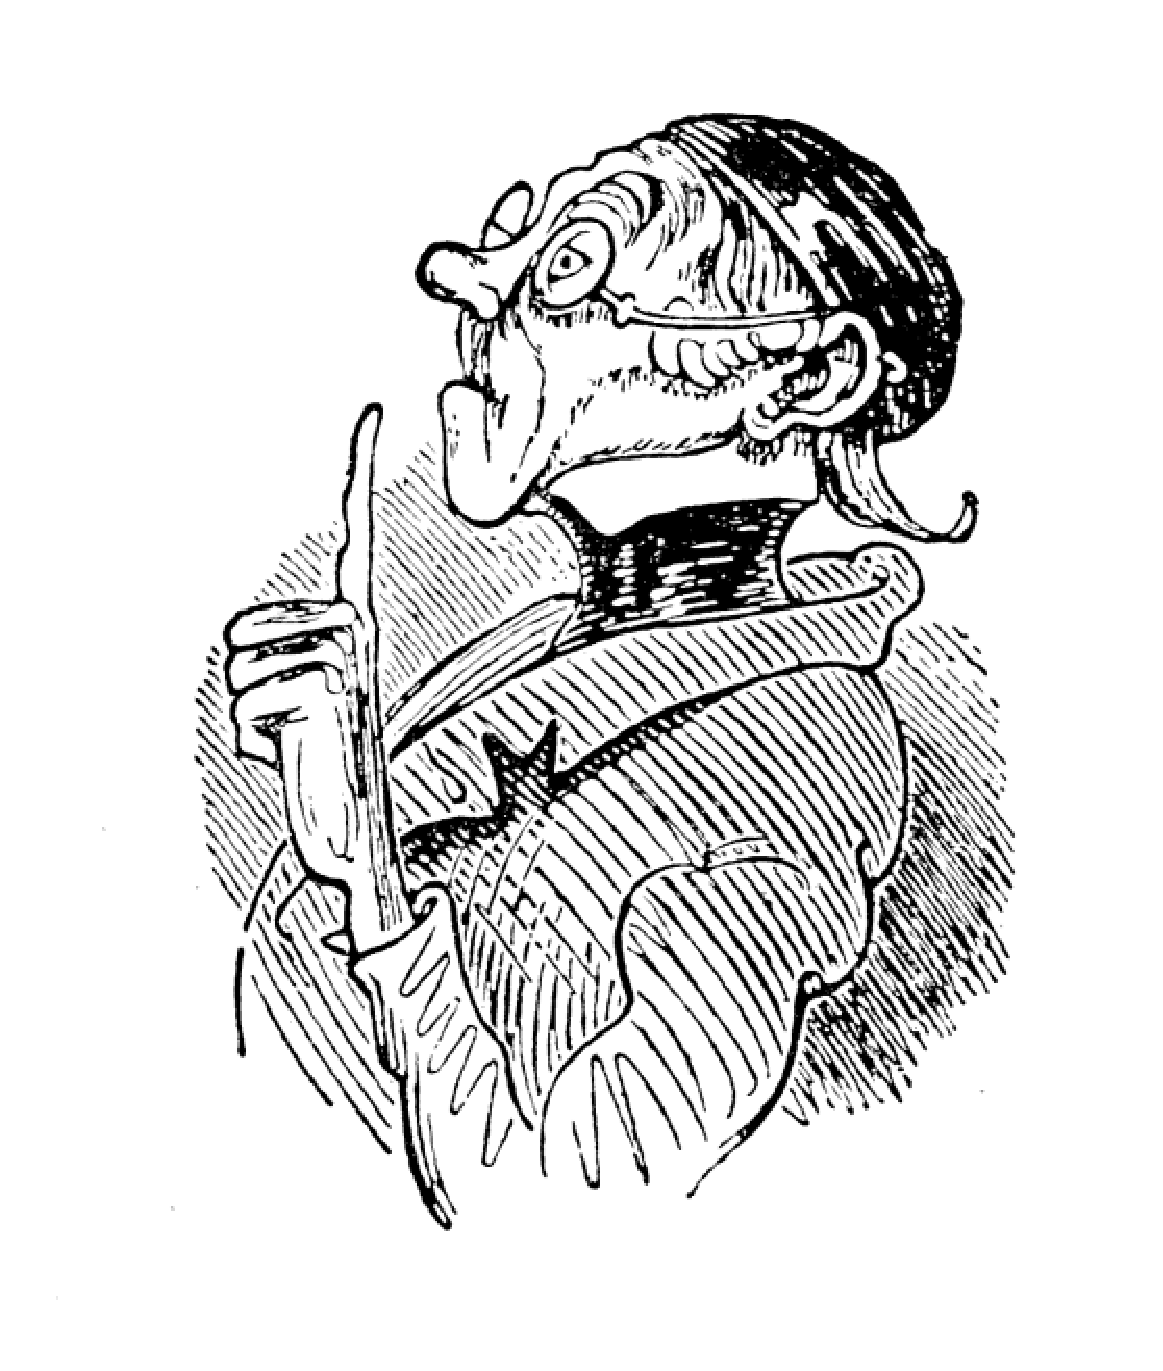
\includegraphics[width=0.75\textwidth]{pics/title_pic.eps}

{\Large \bf Master's Thesis}

\vspace{0.5cm}

{Räuber Hotzenplotz, Matr.-Nr. 1234567} \\
\textbf{Dezember 2013}

\vfill

% table for supervisor and examiners
{\begin{tabular}{ll}
  Supervisor: \hspace{6cm} & Examiners: \\
  Dipl.-Ing. First Name Family Name & Prof. Dr.-Ing. Udo Nackenhorst \\
                                    & Prof. Dr.-Ing. First Name Family Name \\
\end{tabular}}
\end{center}
\end{titlepage}


% Ehrenwörtliche Erklärung
 \pagebreak
\begin{titlepage}

\begin{center}
\textbf{\huge{Ehrenw\"{o}rtliche Erkl\"{a}rung}}
\end{center}

\vspace{3cm}

\noindent Hiermit versichere ich, dass ich die vorliegende Arbeit selbstst\"{a}ndig
verfasst und keine anderen als die angegebenen Quellen und
Hilfsmittel benutzt habe und dass die Arbeit in gleicher oder
\"{a}hnlicher Form noch keiner anderen Pr\"{u}fungsbeh\"{o}rde vorgelegt wurde.



\vspace{5cm}

\hfill
\begin{tabular}{ll}
Hannover, &.........................................\\
\\
\\
\\
\\
  &......................................... \\
  &First Name Family Name \\					% Name
\end{tabular}



\end{titlepage}
		% confirmation of authorship
%\pagebreak
\begin{titlepage}

\begin{center}
\textbf{\huge{Confirmation of Authorship}}
\end{center}

\vspace{3cm}

\noindent I hereby confirm that I have independently composed this Master thesis and that no other than the indicated aid and sources have been used. This work has not been presented to any other examination board.

\vspace{5cm}

\hfill
\begin{tabular}{ll}
Hannover, &.........................................\\
\\
\\
\\
\\
  &......................................... \\
  &First Name Family Name \\					% Name
\end{tabular}




\end{titlepage}
	% confirmation of authorship in ENGLISH 
% \begin{titlepage}
\vspace*{-3.0cm}
\centerline{\includegraphics[width=1.3\textwidth]{./Aufgabenstellung.ps}}
\end{titlepage}
	% include the assignment of tasks
\thispagestyle{empty}
\section*{Abstract}
Insert your abstract here.

% table of contents (automatically)
\pagenumbering{roman}			% roman pagination for table of contents
\tableofcontents
% optional: list of figures
%\listoffigures

\pagenumbering{arabic}
\include{./chapters/01_introduction}
\section{Theory}
\subsection{Figures}
Figures can be inserted as floating objects. They can be arranged in several different ways, dependent on the size and content of the pictures.\\
The \LaTeX{} code for Fig. \ref{fig:1} is
\begin{verbatim}
\begin{figure}[b]
\includegraphics[width=\linewidth, height=2cm]{empty}
\caption{The usual figure environment. It ...}
\label{fig:1}
\end{figure}
\end{verbatim}
%%%%%%%%%%%%%%%%%%%%%%%%%%%%%%%%%%%%%%%
\begin{figure}[b]
\includegraphics[width=\linewidth, height=2cm]{empty}
\caption{The usual figure environment. It may be used for figures spanning the
  whole page width.}
\label{fig:1}
\end{figure}
%%%%%%%%%%%%%%%%%%%%%%%%%%%%%%%%%%%%%%%
Figures should not be inserted without referring to them in the text. Text text text text text text text text text text text text text text text text text text text text text text text text text text text text text text text text text text text text text text text text text text text text text text text text text text text text text text text text text text text text text text text text text text text text text text text text text text text text text text text text text text text text text text text text text text text text text text text text text text text text text text text text text text text text text text text text text text text text text text text text text text text text text text text text text text text text text text text text text text text text text text text text text text text text text text \dots see figure \ref{fig:2}.

Text text text text text text text text text text text text text text text text text text text text text text text text text text text text text text text text text text text text text text text text text text text text text text text text text text text text text text text text text text text text text text text text text text text text text text text text text text text text text text text text text text text text text text text text text text text text text text text text text text text text text text text text text text text text text text text text text text text text text text text text text text text text text text text text \dots as indicated in figure \ref{fig:3}.\\
\dots is plotted in figure \ref{fig:4} and \dots is given in figure \ref{fig:5}.
%%%%%%%%%%%%%%%%%%%%%%%%%%%%%%%%%%%%%%%
\begin{figure}%[b]
  \includegraphics[width=.5\textwidth,height=25mm]{empty}
\caption{A figure  environment with a caption.
Figure and caption are leftindented.}
\label{fig:2}
\end{figure}
%%%%%%%%%%%%%%%%%%%%%%%%%%%%%%%%%%%%%%%

Two small pictures can be located side by side, to avoid plenty of free space. An example is given in figures \ref{fig:3} and \ref{fig:4}.
%%%%%%%%%%%%%%%%%%%%%%%%%%%%%%%%%%%%%%%
\begin{figure}
\begin{minipage}{72mm}
\includegraphics[width=\linewidth,height=25mm]{empty}
\caption{Two figures side by side with different numbers.}
\label{fig:3}
\end{minipage}
\hfil
\begin{minipage}{65mm}
\includegraphics[width=\linewidth,height=25mm]{empty}
\caption{This is the second picture.}
\label{fig:4}
\end{minipage}
\end{figure}
%%%%%%%%%%%%%%%%%%%%%%%%%%%%%%%%%%%%%%%

If two pictures belong together, they can be arranged in one \verb+\figure+ environment with a joint caption.
%%%%%%%%%%%%%%%%%%%%%%%%%%%%%%%%%%%%%%%
\begin{figure}
\includegraphics[width=68mm,height=25mm]{empty}~a)
\hfil
\includegraphics[width=68mm,height=25mm]{empty}~b)
\caption{Two figures with one number. The figures are referred to as \textbf{a}
and \textbf{b}.}
\label{fig:5}
\end{figure}
%%%%%%%%%%%%%%%%%%%%%%%%%%%%%%%%%%%%%%%

It should be made sure that it is not only referred to every picture in the text, but that every picture is also discussed.\\
x is plotted against y\dots The dotted line, the broken line, the solid line \dots The limb of the curve \dots\\
The crest, the peak, the trough, rising sharply, \dots
%%%%%%%%%%%%%%%%%%%%%%%%%%%%%%%%%%%%%%%
\subsection{Test of math environments}
Equations are always left-aligned. Therefore the option {fleqn} is used for the
documentclass command by default. Note that {fleqn} does not work with
unnumbered displayed equations written as \verb+$$ Ax =b $$+, so please use
\verb+\[ Ax=b \]+ or an \texttt{equation*} or \texttt{gather*} environment
instead.

By default the equations are consecutively numbered. This may be changed by
putting the following command inside the preamble
\begin{center}
  \verb+\numberwithin{equation}{section}+
\end{center}

The latex math display environment \verb+\[+\ldots\verb+\]+
\[
  \sum_{i=1}^{\infty} \frac{1}{i^2}
\]

An equation environment:
\begin{equation}
  \label{eq:eq}
  \sum_{i=1}^{\infty} \frac{1}{i^2}
\end{equation}
For more mathematical commands and environments please refer to the documentation of the \AmS{} classes. Search the internet, the wikipedia.de \TeX--help or consult the book \cite{sturm2007}.
%%%%%%%%%%%%%%%%%%%%%%%%%%%%%%%%%%%%%%%
\subsection{Literature}
Insert references to the relevant literature into the text. Futhermore make sure that all content from any external source is marked as such properly. References or citations can be used at the discretion of the author, as long as they are marked properly.\\
\cite{oden_reddy_2011}\\
\cite{nackenhorst_2004}\\
\cite{holzapfel_2000}\\
\cite{zienkiewicz_taylor_1989}\\
\cite{ziefle_2008}\\
\cite{sagar_2010}
\section{My Developments}
\subsection{Tables}
\dots is given in table \ref{table:1} \ldots
\begin{table}[h]
  \caption{this my nice table}
  \label{table:1}
  \begin{center}
  \begin{tabular}{@{}lrcp{3cm}}
  \toprule
    left-aligned & right-aligned & centered     & user-defined column width\\
  \midrule
    ---        & mm           & mm            & of 3 cm!\\
  \midrule
    element    & 0,289376670  &  0,289376679  & $-9,0 \cdot 10^{-9}$\\
    \multicolumn{3}{c}{this item merges 3 columns}\\
    ele        & 0,28         &  0,28         & automatical line break due to wide item\\
    eleme      & 0,28         &  0,28         & $-8,0 \cdot 10^{-9}$\\
  \bottomrule
  \end{tabular}
  \end{center}
\end{table}
\include{./chapters/04_implementation}
\section{Numerical Examples}
Matlab code can be embedded like this:
\begin{lstlisting}
% Example Matlab code for calculating hypotenuse
% § $c = \sqrt{a^2+b^2}$ §
a = 3;
b = 4;
c = sqrt(a^2+b^2);
\end{lstlisting}
or like this:
\lstinputlisting{./pathtomymfile/myfile.m}
\include{./chapters/06_conclusion}

% list of references (automatically)

\thispagestyle{plain}
% \bibliographystyle{apalike}		% reference: author, (year), title (ENGLISH), alphabetically 
\bibliographystyle{plain}		% reference: number, author, title, year (ENGLISH),alphabetically 
 %\bibliographystyle{dinat}		% reference: author in small caps, title, year,(DEUTSCH), alphabetically
% \bibliographystyle{natdin}		% reference: author in small caps, title, year,(DEUTSCH), alphabetically
\bibliography{mybib}

\end{document}



